%
% Documento: Fundamentação Teórica
%

\chapter{Elementos flutuantes, equações e referências cruzadas}
\label{chap:ef}

A seguir ilustra-se a forma de incluir figuras, tabelas, equações, siglas e 
símbolos no documento, obtendo indexação automática em suas respectivas
                listas.
A numeração sequencial de figuras, tabelas e equações ocorre de modo automático.
Referências cruzadas são obtidas através dos comandos \verb#\label{}# e \verb#\ref{}#.
Por exemplo, não é necessário saber que o número deste capítulo é \ref{chap:ef} para colocar o seu número no texto.
Isto facilita muito a inserção, remoção ou relocação de elementos numerados no texto (fato corriqueiro na escrita e correção de um documento acadêmico) sem a necessidade de renumerá-los todos.





 
\section{Equações}
\label{sec:equacoes}

A transformada de Laplace é dada na \autoref{eq:laplace}, enquanto a \autoref{eq:dft} apresenta a formulação da transformada discreta de Fourier bidimensional\footnote{Deve-se reparar na formatação esteticamente perfeita destas equações.}.


\begin{equation}
    X(s) = \int\limits_{t = -\infty}^{\infty} x(t) \, \text{e}^{-st} \, dt
    \label{eq:laplace}
\end{equation}

\begin{equation}
    F(u, v) = \sum_{m = 0}^{M - 1} \sum_{n = 0}^{N - 1} f(m, n) \exp \left[ -j 2 \pi \left( \frac{u m}{M} + \frac{v n}{N} \right) \right]
    \label{eq:dft}
\end{equation}


\section{Elementos flutuantes (tabelas, quadros, gráficos e figuras)}

Tabelas, quadros, gráficos e figuras são elementos utilizados em trabalhos acadêmicos, e possuem diferenças e especificações definidas pela ABNT.

As tabelas são formadas por linhas verticais, devem manter suas bordas laterais abertas e geralmente são utilizadas para dados quantitativos. Os quadros, por outro lado, são formados por linhas verticais e horizontais, devem ter todas suas extremidades fechadas e são mais utilizados para dados qualitativos.

Por último, as figuras e gráficos são elementos ilustrativos, que podem ser em forma de fotos, mapas, gráficos, gravuras, etc.

Todos estes elementos devem estar centralizados, com legenda na parte superior e fonte na parte inferior (ver Quadro \ref{quadroex1} para maiores detalhes).

De forma geral, esses ambiantes podem ser utilizados com os seguintes comandos



\begin{verbatim}
\begin{nome do ambiente}[H]
   \centering
   \caption{legenda}
   \label{"etiqueta"}
      inserção do elemento 
   \fonte{fonte do elemento}
\end{table}
\end{verbatim}
Os campos apresentados nos códigos acima estão explicados no Quadro \ref{quadroex2}.


\begin{quadro}[H]
	\centering
	\caption{Alguns detalhes sobre elementos flutuantes}
	\label{quadroex1}
	\begin{tabular}{|l|m{4cm}|m{4cm}|m{4cm}|}
		\hline
		& \textbf{Tabela}                                                                             & \textbf{Quadro}                                                                             & \textbf{Figuras}                                                                    \\ \hline
		\textbf{Formato}    & Bordas laterais não podem ser fechadas.                                                     & As extremidades devem ser fechadas.                                                         & Podem ser em forma de fotos, mapas, gráficos, gravuras, etc.                        \\ \hline
		\textbf{Uso}        & Geralmente para dados quantitativos.                                                        & Geralmente para dados qualitativos.                                                         & Ilustrar informações e dados.                                                       \\ \hline
		\textbf{Elementos}  & Título, cabeçalho, conteúdo, fonte e, se necessário, notas explicativas.                    & Título, fonte, legenda e notas.                                                             & Título, numeração e fonte.                                                          \\ \hline
		\textbf{Divisão}    & Formada por linhas verticais.                                                               & Formado por linhas horizontais e verticais.                                                 & -                                                                                   \\ \hline
		\textbf{Formatação} & O número e o título da tabela devem vir acima dela, enquanto a fonte deve aparecer embaixo. & O número e o título do quadro devem vir acima dele, enquanto a fonte deve aparecer embaixo. & O número e o título devem aparecer no topo, enquanto a fonte deve aparecer embaixo. \\ \hline
	\end{tabular}
	\fonte{\citeonline{diana}}
\end{quadro}

\begin{quadro}[H]
	\centering
	\caption{Alguns campos utilizados em elementos flutuantes}
	\label{quadroex2}
	\begin{tabular}{|m{4cm}|m{8cm}|}
		\hline
	\verb|nome do ambiente| & \verb|figure|: para figuras, \verb|grafico|: para gráficos, \verb|table|: para tabelas e \verb|quadro|: para quadros\\ \hline
	\verb|legenda| & Deve ser inserida como argumento no comando \verb|\caption{}| e refere-se a legenda do elemento flutuante.\\ \hline
	\verb|"etiqueta"| & Deve ser inserida como argumento no comando \verb|\label{}| e consiste em um nome dado para referenciarmos àquele elemento flutuante no texto.\\ \hline
	\verb|fonte do elemento| & Deve ser inserida como argumento no comando \verb|\fonte{}| e consiste da informação de onde retirou-se o elemento.\\ \hline
	\end{tabular}
	\fonte{Elaborado pelo autor}
\end{quadro}


Abaixo apresentamos alguns exemplos de outros elementos flutuantes  seguidos dos códigos utilizados para inseri-los.

A Figura \ref{fig:conceitodt} aparece automaticamente na lista de figuras.
Para uso avançado de imagens no \LaTeX, recomenda-se a consulta de literatura especializada \cite{Goossens2007}.

\begin{figure}[H]
	\centering
	\caption{Ilustração do conceito de derivada topológica.}
	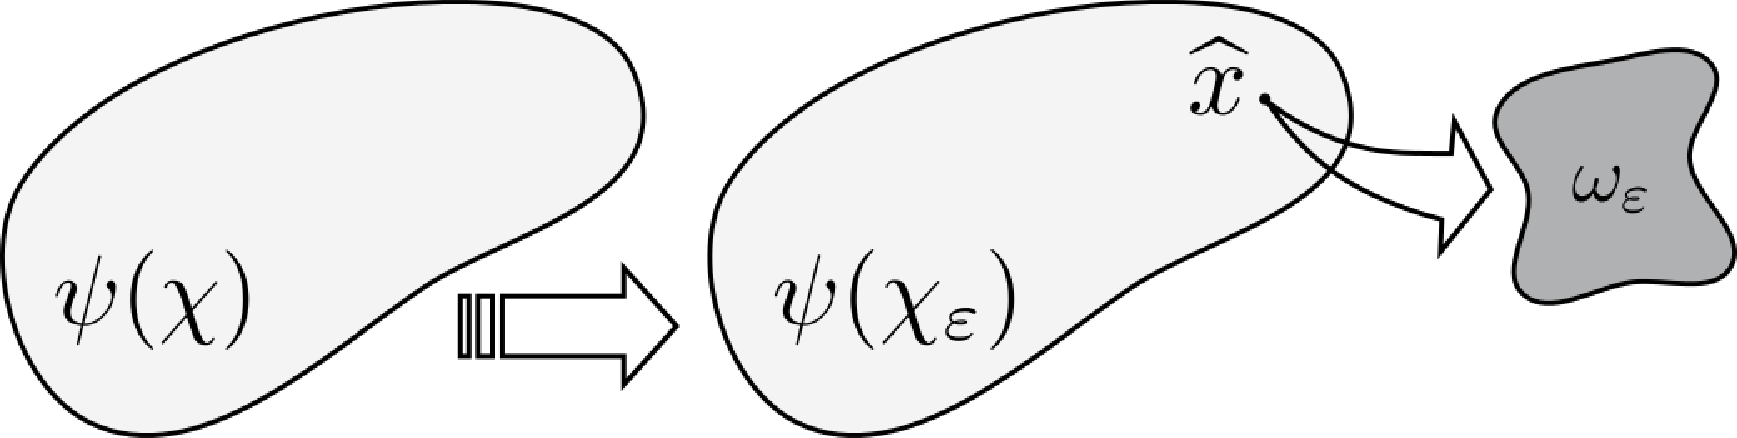
\includegraphics[width=0.6\textwidth]{./figuras/conceito.pdf}
	\fonte{\citeonline{NovotnyBook2013}}
	\label{fig:conceitodt}
\end{figure}

\begin{verbatim}
\begin{figure}[H]
  \centering
  \caption{Conceito de derivada topológica.}
    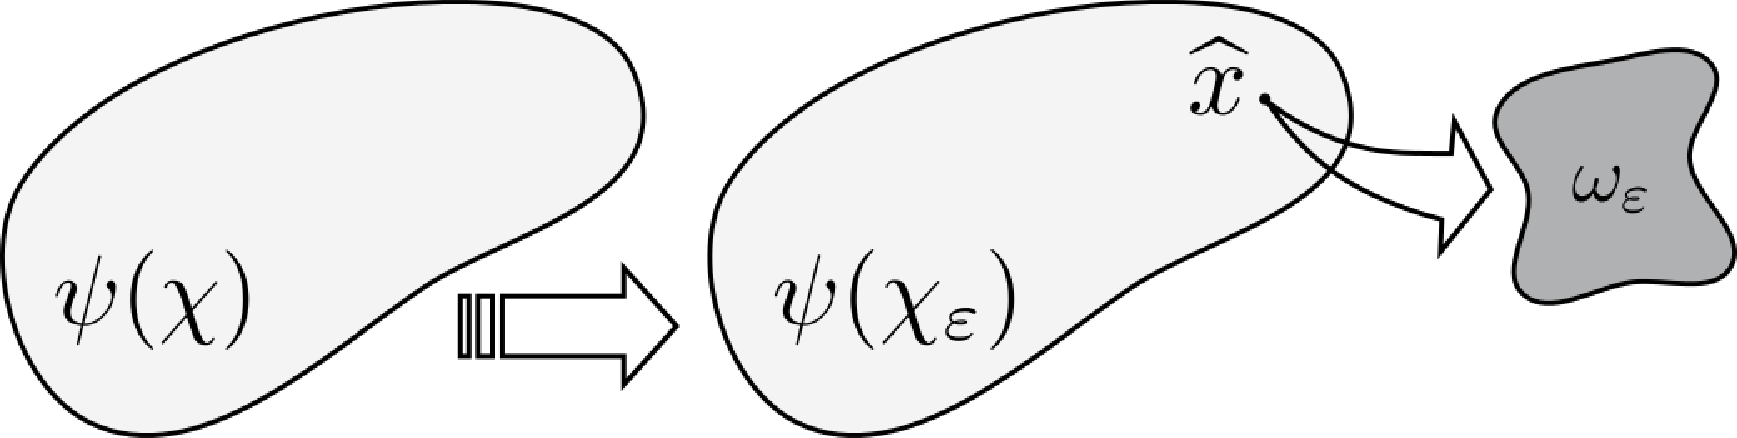
\includegraphics[width=0.6\textwidth]{./figuras/conceito.pdf}
  \fonte{\citeonline{NovotnyBook2013}}
  \label{fig:conceitodt}
\end{figure}
\end{verbatim}


\begin{table}[H]
\centering
\caption{Um nome qualquer}
\label{ExemploTab}
\begin{tabular}{r|lr}	
Posição & País & IDH \\ \hline
	1 & Noruega        & .955 \\
	2 & Austrália  & .938 \\
	3 & EUA            & .937 \\
	4 & Holanda        & .921 \\
	5 & Alemanha       & .920            % não é preciso quebrar a última linha
\end{tabular}
% \fonte{\citeonline{garcia}}
\end{table}




\begin{verbatim}
\begin{table}[H]
\centering
\caption{Um nome qualquer}
\label{ExemploTab}
\begin{tabular}{r|lr}	
    	Posição & País & IDH \\	\hline
    	1 & Noruega        & .955 \\
    	2 & Austrália  & .938 \\
    	3 & EUA            & .937 \\
    	4 & Holanda        & .921 \\
    	5 & Alemanha       & .920 
\end{tabular}
\fonte{\citeonline{garcia}}
\end{table}
\end{verbatim}


\pagebreak

No Gráfico \ref{gr:exgrafico} apresentamos um exemplo de gráfico.

\begin{grafico}[H]
\centering
\caption{Evolução de matrículas dos Institutos Federais}
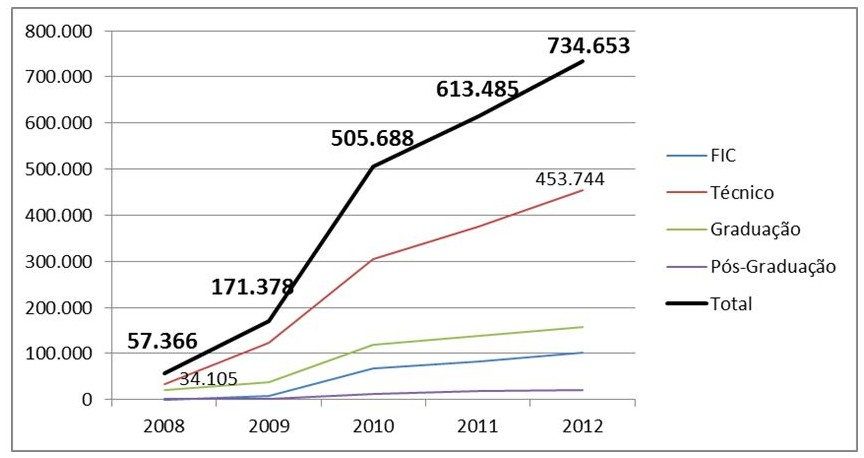
\includegraphics[height=6cm]{./figuras/redefederal.jpg}	
\fonte{MEC/SETEC}
\label{gr:exgrafico}
\end{grafico}

\begin{verbatim}
\begin{grafico}[H]
  \centering
  \caption{Evolução de matrículas dos Institutos Federais}
    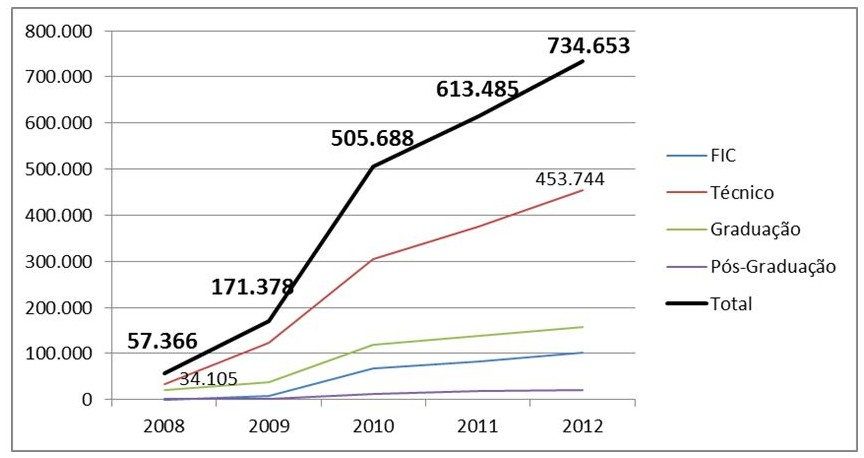
\includegraphics[height=6cm]{./figuras/redefederal.jpg}	
  \fonte{MEC/SETEC}
  \label{gr:exgrafico}
\end{grafico}
\end{verbatim}